% GNUPLOT: LaTeX picture with Postscript
\begingroup
  \makeatletter
  \providecommand\color[2][]{%
    \GenericError{(gnuplot) \space\space\space\@spaces}{%
      Package color not loaded in conjunction with
      terminal option `colourtext'%
    }{See the gnuplot documentation for explanation.%
    }{Either use 'blacktext' in gnuplot or load the package
      color.sty in LaTeX.}%
    \renewcommand\color[2][]{}%
  }%
  \providecommand\includegraphics[2][]{%
    \GenericError{(gnuplot) \space\space\space\@spaces}{%
      Package graphicx or graphics not loaded%
    }{See the gnuplot documentation for explanation.%
    }{The gnuplot epslatex terminal needs graphicx.sty or graphics.sty.}%
    \renewcommand\includegraphics[2][]{}%
  }%
  \providecommand\rotatebox[2]{#2}%
  \@ifundefined{ifGPcolor}{%
    \newif\ifGPcolor
    \GPcolortrue
  }{}%
  \@ifundefined{ifGPblacktext}{%
    \newif\ifGPblacktext
    \GPblacktextfalse
  }{}%
  % define a \g@addto@macro without @ in the name:
  \let\gplgaddtomacro\g@addto@macro
  % define empty templates for all commands taking text:
  \gdef\gplbacktext{}%
  \gdef\gplfronttext{}%
  \makeatother
  \ifGPblacktext
    % no textcolor at all
    \def\colorrgb#1{}%
    \def\colorgray#1{}%
  \else
    % gray or color?
    \ifGPcolor
      \def\colorrgb#1{\color[rgb]{#1}}%
      \def\colorgray#1{\color[gray]{#1}}%
      \expandafter\def\csname LTw\endcsname{\color{white}}%
      \expandafter\def\csname LTb\endcsname{\color{black}}%
      \expandafter\def\csname LTa\endcsname{\color{black}}%
      \expandafter\def\csname LT0\endcsname{\color[rgb]{1,0,0}}%
      \expandafter\def\csname LT1\endcsname{\color[rgb]{0,1,0}}%
      \expandafter\def\csname LT2\endcsname{\color[rgb]{0,0,1}}%
      \expandafter\def\csname LT3\endcsname{\color[rgb]{1,0,1}}%
      \expandafter\def\csname LT4\endcsname{\color[rgb]{0,1,1}}%
      \expandafter\def\csname LT5\endcsname{\color[rgb]{1,1,0}}%
      \expandafter\def\csname LT6\endcsname{\color[rgb]{0,0,0}}%
      \expandafter\def\csname LT7\endcsname{\color[rgb]{1,0.3,0}}%
      \expandafter\def\csname LT8\endcsname{\color[rgb]{0.5,0.5,0.5}}%
    \else
      % gray
      \def\colorrgb#1{\color{black}}%
      \def\colorgray#1{\color[gray]{#1}}%
      \expandafter\def\csname LTw\endcsname{\color{white}}%
      \expandafter\def\csname LTb\endcsname{\color{black}}%
      \expandafter\def\csname LTa\endcsname{\color{black}}%
      \expandafter\def\csname LT0\endcsname{\color{black}}%
      \expandafter\def\csname LT1\endcsname{\color{black}}%
      \expandafter\def\csname LT2\endcsname{\color{black}}%
      \expandafter\def\csname LT3\endcsname{\color{black}}%
      \expandafter\def\csname LT4\endcsname{\color{black}}%
      \expandafter\def\csname LT5\endcsname{\color{black}}%
      \expandafter\def\csname LT6\endcsname{\color{black}}%
      \expandafter\def\csname LT7\endcsname{\color{black}}%
      \expandafter\def\csname LT8\endcsname{\color{black}}%
    \fi
  \fi
    \setlength{\unitlength}{0.0500bp}%
    \ifx\gptboxheight\undefined%
      \newlength{\gptboxheight}%
      \newlength{\gptboxwidth}%
      \newsavebox{\gptboxtext}%
    \fi%
    \setlength{\fboxrule}{0.5pt}%
    \setlength{\fboxsep}{1pt}%
\begin{picture}(7360.00,2820.00)%
    \gplgaddtomacro\gplbacktext{%
      \csname LTb\endcsname%%
      \put(498,396){\makebox(0,0)[r]{\strut{}\footnotesize$10^{0}$}}%
      \csname LTb\endcsname%%
      \put(498,1080){\makebox(0,0)[r]{\strut{}\footnotesize$10^{1}$}}%
      \csname LTb\endcsname%%
      \put(498,1763){\makebox(0,0)[r]{\strut{}\footnotesize$10^{2}$}}%
      \csname LTb\endcsname%%
      \put(498,2447){\makebox(0,0)[r]{\strut{}\footnotesize$10^{3}$}}%
      \csname LTb\endcsname%%
      \put(566,248){\makebox(0,0){\strut{}\footnotesize$10^{-3}$}}%
      \csname LTb\endcsname%%
      \put(1127,248){\makebox(0,0){\strut{}\footnotesize$10^{-2}$}}%
      \csname LTb\endcsname%%
      \put(1688,248){\makebox(0,0){\strut{}\footnotesize$10^{-1}$}}%
      \csname LTb\endcsname%%
      \put(2249,248){\makebox(0,0){\strut{}\footnotesize$10^{0}$}}%
    }%
    \gplgaddtomacro\gplfronttext{%
      \csname LTb\endcsname%%
      \put(102,1421){\rotatebox{-270}{\makebox(0,0){\strut{}\small selectivity}}}%
      \csname LTb\endcsname%%
      \put(1407,86){\makebox(0,0){\strut{}\small pressure / bar}}%
      \csname LTb\endcsname%%
      \put(1407,2633){\makebox(0,0){\strut{}\ce{C3H8} / \ce{C2H6}}}%
      \csname LTb\endcsname%%
      \put(1382,2305){\makebox(0,0)[r]{\strut{}\footnotesize$y_{\smallce{C3}} = 0.1$}}%
      \csname LTb\endcsname%%
      \put(1382,2119){\makebox(0,0)[r]{\strut{}\footnotesize$y_{\smallce{C3}} = 0.5$}}%
      \csname LTb\endcsname%%
      \put(1382,1933){\makebox(0,0)[r]{\strut{}\footnotesize$y_{\smallce{C3}} = 0.9$}}%
    }%
    \gplgaddtomacro\gplbacktext{%
      \csname LTb\endcsname%%
      \put(2827,396){\makebox(0,0)[r]{\strut{}\footnotesize$10^{0}$}}%
      \csname LTb\endcsname%%
      \put(2827,1422){\makebox(0,0)[r]{\strut{}\footnotesize$10^{1}$}}%
      \csname LTb\endcsname%%
      \put(2827,2447){\makebox(0,0)[r]{\strut{}\footnotesize$10^{2}$}}%
      \csname LTb\endcsname%%
      \put(2895,248){\makebox(0,0){\strut{}\footnotesize$10^{-3}$}}%
      \csname LTb\endcsname%%
      \put(3497,248){\makebox(0,0){\strut{}\footnotesize$10^{-2}$}}%
      \csname LTb\endcsname%%
      \put(4100,248){\makebox(0,0){\strut{}\footnotesize$10^{-1}$}}%
      \csname LTb\endcsname%%
      \put(4702,248){\makebox(0,0){\strut{}\footnotesize$10^{0}$}}%
    }%
    \gplgaddtomacro\gplfronttext{%
      \csname LTb\endcsname%%
      \put(3798,86){\makebox(0,0){\strut{}\small pressure / bar}}%
      \csname LTb\endcsname%%
      \put(3798,2633){\makebox(0,0){\strut{}\ce{C4H10} / \ce{C3H8}}}%
      \csname LTb\endcsname%%
      \put(4381,2305){\makebox(0,0)[r]{\strut{}\footnotesize$y_{\smallce{C4}} = 0.1$}}%
      \csname LTb\endcsname%%
      \put(4381,2119){\makebox(0,0)[r]{\strut{}\footnotesize$y_{\smallce{C4}} = 0.5$}}%
      \csname LTb\endcsname%%
      \put(4381,1933){\makebox(0,0)[r]{\strut{}\footnotesize$y_{\smallce{C4}} = 0.9$}}%
    }%
    \gplgaddtomacro\gplbacktext{%
      \csname LTb\endcsname%%
      \put(5280,396){\makebox(0,0)[r]{\strut{}\footnotesize$10^{1}$}}%
      \csname LTb\endcsname%%
      \put(5280,1080){\makebox(0,0)[r]{\strut{}\footnotesize$10^{2}$}}%
      \csname LTb\endcsname%%
      \put(5280,1763){\makebox(0,0)[r]{\strut{}\footnotesize$10^{3}$}}%
      \csname LTb\endcsname%%
      \put(5280,2447){\makebox(0,0)[r]{\strut{}\footnotesize$10^{4}$}}%
      \csname LTb\endcsname%%
      \put(5348,248){\makebox(0,0){\strut{}\footnotesize$10^{-3}$}}%
      \csname LTb\endcsname%%
      \put(5950,248){\makebox(0,0){\strut{}\footnotesize$10^{-2}$}}%
      \csname LTb\endcsname%%
      \put(6553,248){\makebox(0,0){\strut{}\footnotesize$10^{-1}$}}%
      \csname LTb\endcsname%%
      \put(7155,248){\makebox(0,0){\strut{}\footnotesize$10^{0}$}}%
    }%
    \gplgaddtomacro\gplfronttext{%
      \csname LTb\endcsname%%
      \put(6251,86){\makebox(0,0){\strut{}\small pressure / bar}}%
      \csname LTb\endcsname%%
      \put(6251,2633){\makebox(0,0){\strut{}\ce{C4H10} / \ce{C2H6}}}%
      \csname LTb\endcsname%%
      \put(6499,2305){\makebox(0,0)[r]{\strut{}\footnotesize$y_{\smallce{C4}} = 0.1$}}%
      \csname LTb\endcsname%%
      \put(6499,2119){\makebox(0,0)[r]{\strut{}\footnotesize$y_{\smallce{C4}} = 0.5$}}%
      \csname LTb\endcsname%%
      \put(6499,1933){\makebox(0,0)[r]{\strut{}\footnotesize$y_{\smallce{C4}} = 0.9$}}%
    }%
    \gplbacktext
    \put(0,0){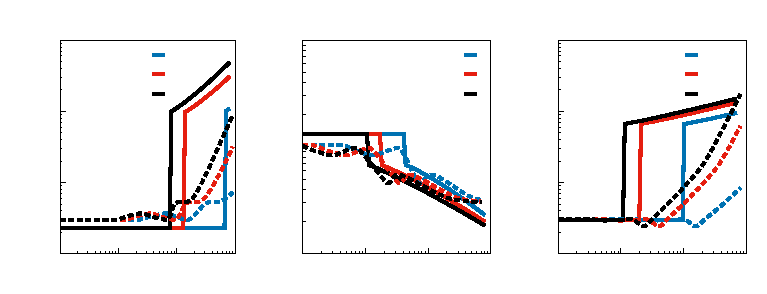
\includegraphics{rpm3-zn-selectivities}}%
    \gplfronttext
  \end{picture}%
\endgroup
